\documentclass[tikz,border=3mm]{standalone}
\usepackage{pgfplots}
\pgfplotsset{compat=1.17}
\usepgfplotslibrary{groupplots}
\begin{document}
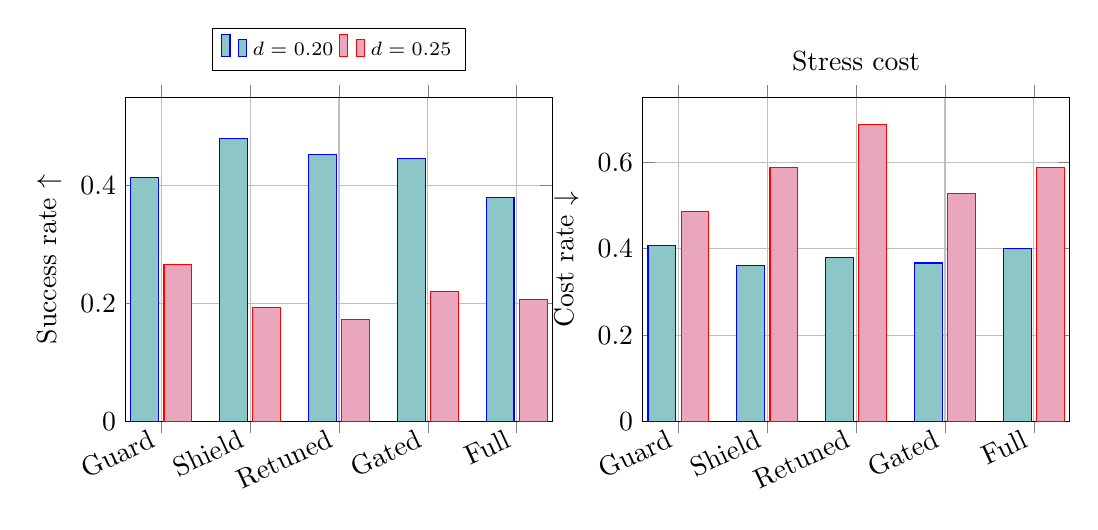
\begin{tikzpicture}
\begin{groupplot}[group style={group size=2 by 1, horizontal sep=1.15cm}, width=7cm, height=5.7cm, ybar, symbolic x coords={Guard,Shield,Retuned,Gated,Full}, xtick=data, x tick label style={rotate=25,anchor=east}, grid=major, legend style={at={(0.5,1.08)},anchor=south,legend columns=2,font=\scriptsize}]
\nextgroupplot[ylabel={Success rate $\uparrow$}, ymin=0,ymax=0.55, title={Stress success}]
\addplot+[fill=teal!45] coordinates {(Guard,0.4133) (Shield,0.4800) (Retuned,0.4533) (Gated,0.4467) (Full,0.3800)}; \addlegendentry{$d=0.20$}
\addplot+[fill=purple!35] coordinates {(Guard,0.2667) (Shield,0.1933) (Retuned,0.1733) (Gated,0.2200) (Full,0.2067)}; \addlegendentry{$d=0.25$}
\nextgroupplot[ylabel={Cost rate $\downarrow$}, ymin=0,ymax=0.75, title={Stress cost}]
\addplot+[fill=teal!45] coordinates {(Guard,0.4067) (Shield,0.3600) (Retuned,0.3800) (Gated,0.3667) (Full,0.4000)};
\addplot+[fill=purple!35] coordinates {(Guard,0.4867) (Shield,0.5867) (Retuned,0.6867) (Gated,0.5267) (Full,0.5867)};
\end{groupplot}
\end{tikzpicture}
\end{document}
